\subsubsection{a and b}

The plots of the logarithm of base 10 of the absolute- and relative error is found in Fig. \ref{task8ab}. 

\begin{figure}
    \centering
    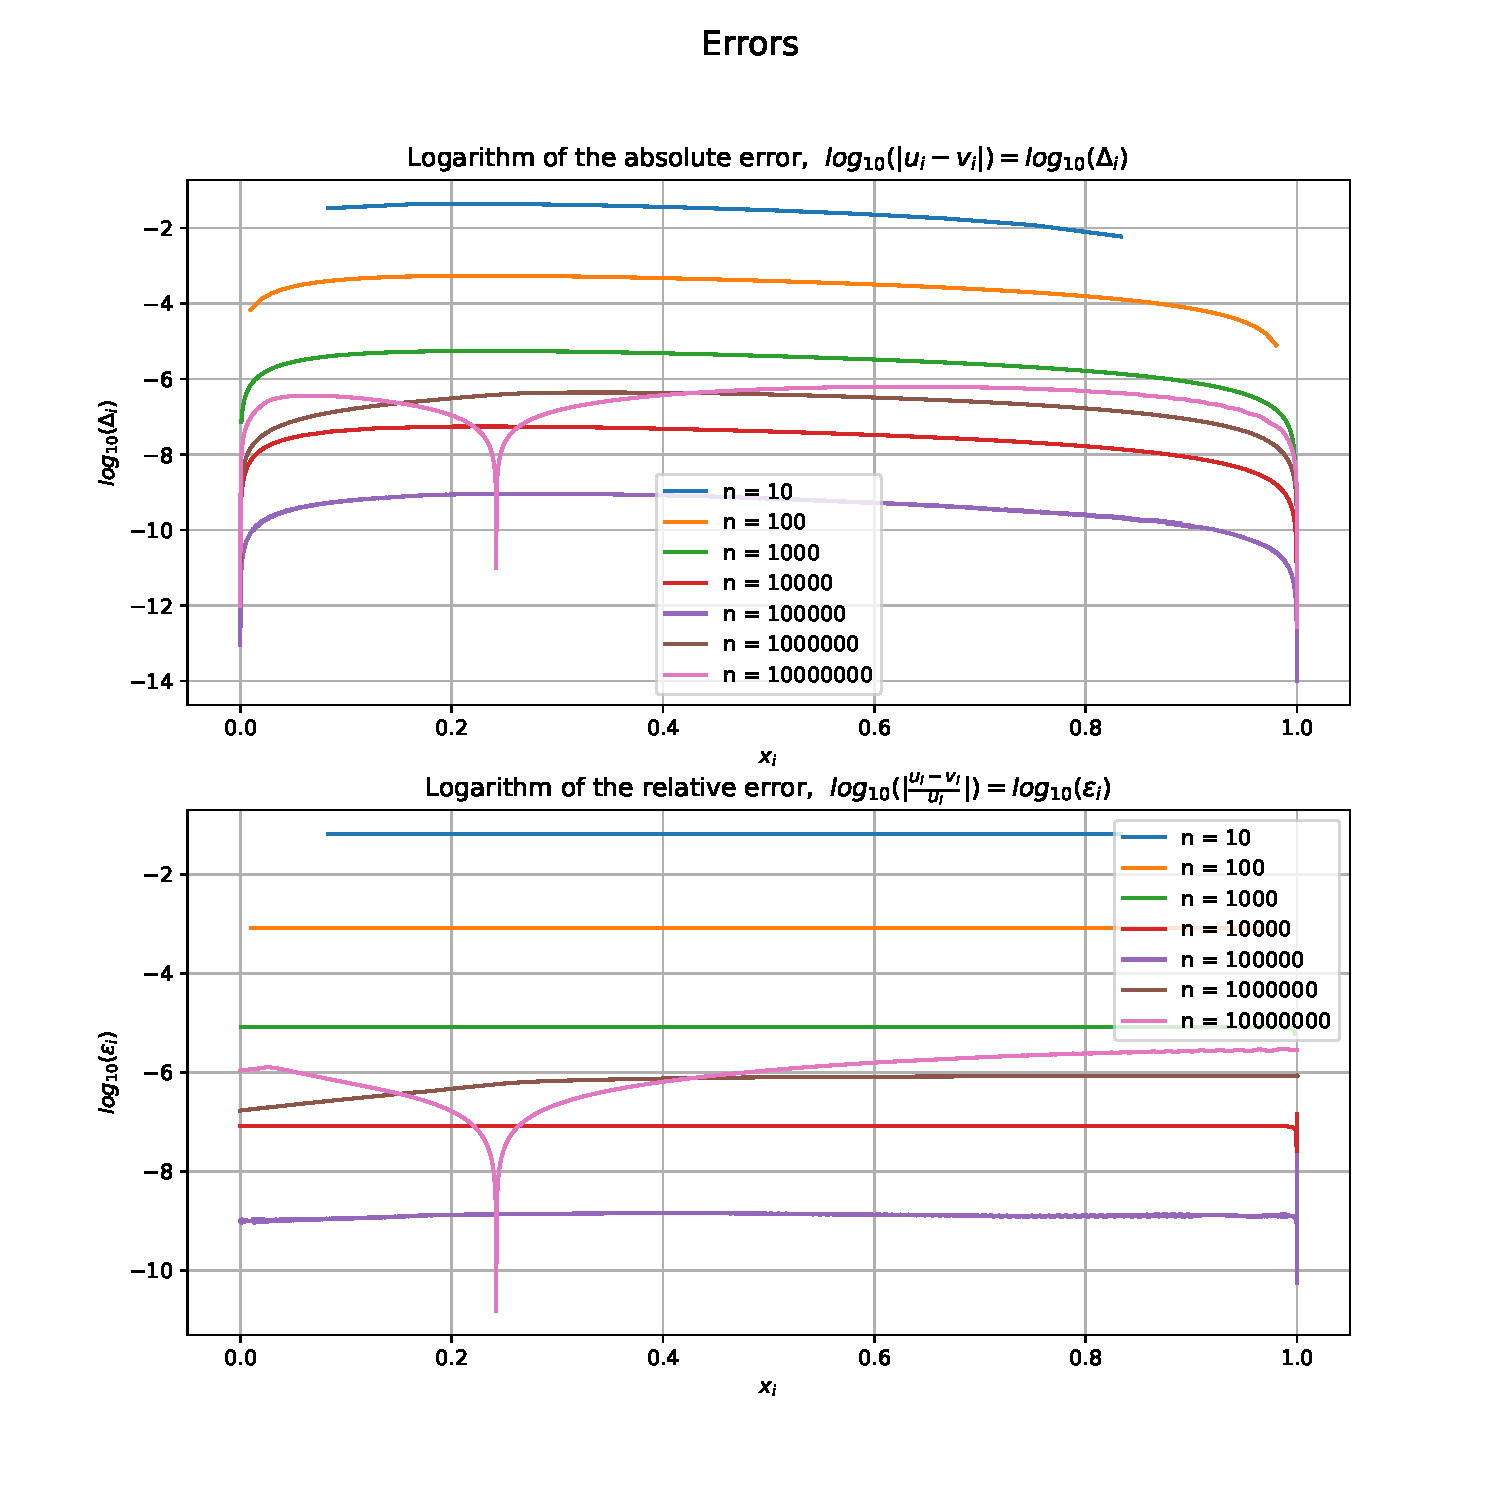
\includegraphics[width=0.5\linewidth]{plot_8.pdf}
    \caption{Show the respective errors for different choices of $n_{steps}$. Since the two boundary points are fixed (u(0) and u(1)), those points are left out in this error analysis.}
    \label{fig:task8ab}
\end{figure}


\subsubsection{c}
Table \ref{tab:table8c} shows the maximum relative error $max(\epsilon_i)$ for each choice of $n_{steps}$. The plot is found in Fig. \ref{task8c} 

\begin{figure}
    \centering
    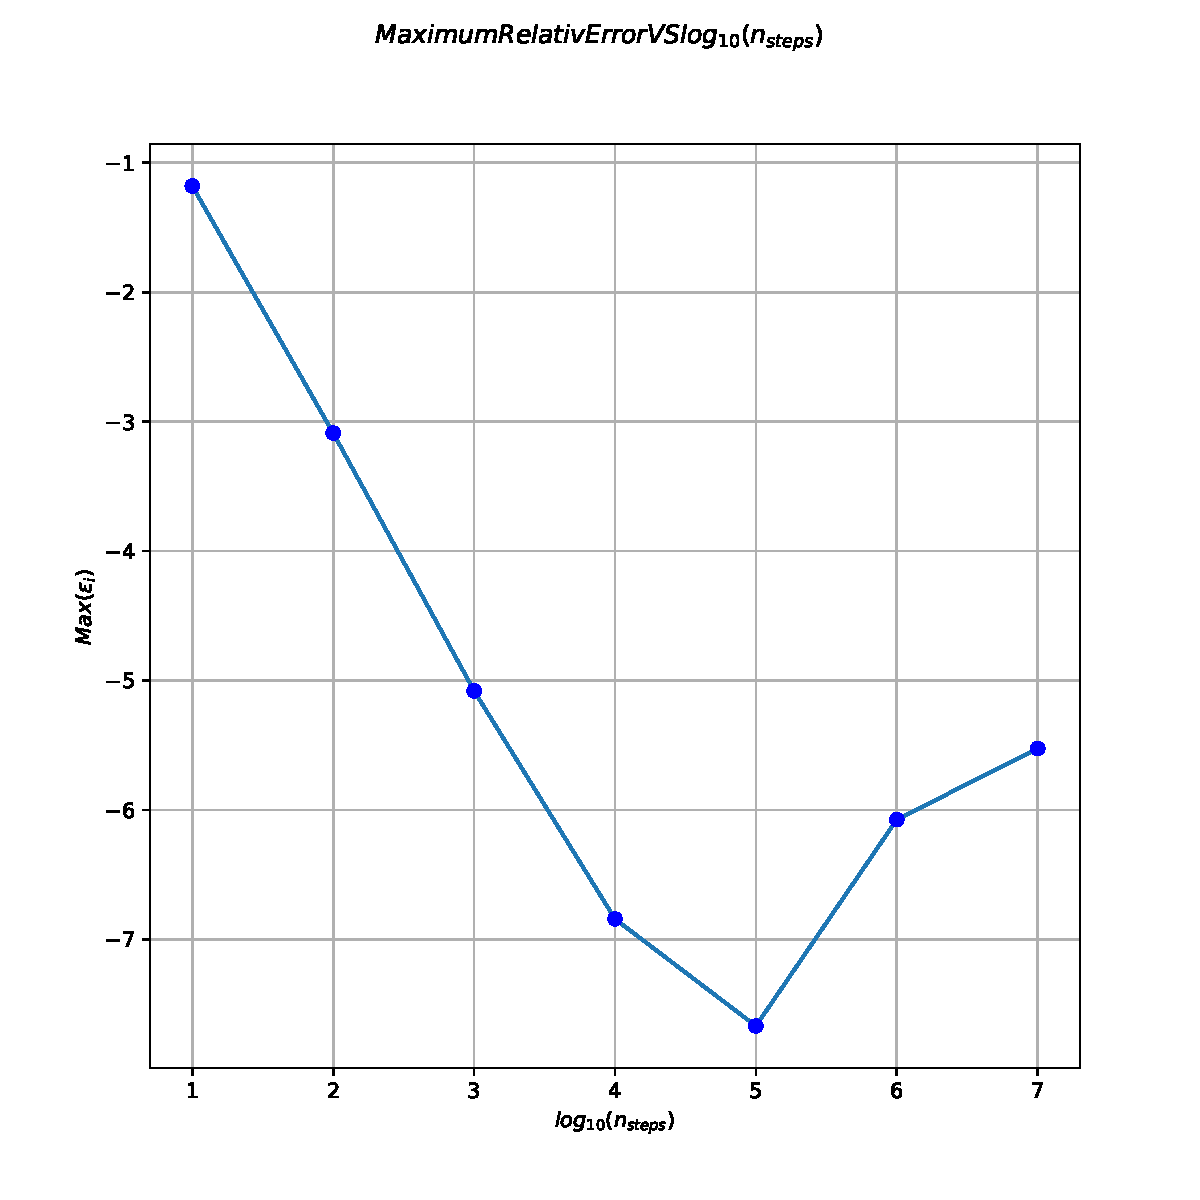
\includegraphics[width=0.5\linewidth]{plot_8_max.pdf}
    \caption{Maximum relative error $max(\epsilon_i)$ for each choice of $n_{steps}$}
    \label{fig:task8c}
\end{figure}

\begin{table}[]
    \centering
    \begin{tabular}{|c|c|}
        \hline
        $n_{steps}$ & $\max(\epsilon_i)$ \\ \hline
        $10^{1}$ & $-1.18$ \\ \hline
        $10^{2}$ & $-3.09$ \\ \hline
        $10^{3}$ & $-5.08$ \\ \hline
        $10^{4}$ & $-6.84$ \\ \hline
        $10^{5}$ & $-7.67$ \\ \hline
        $10^{6}$ & $-6.07$ \\ \hline
        $10^{7}$ & $-5.53$ \\ \hline
        
    \end{tabular}
    \caption{Table of $\log_{10}(n_{steps})$ and maximum $\epsilon_i$}
    \label{tab:table8c}
\end{table}


